%% 
%% Copyright 2007, 2008, 2009 Elsevier Ltd
%% 
%% This file is part of the 'Elsarticle Bundle'.
%% ---------------------------------------------
%% 
%% It may be distributed under the conditions of the LaTeX Project Public
%% License, either version 1.2 of this license or (at your option) any
%% later version.  The latest version of this license is in
%%    http://www.latex-project.org/lppl.txt
%% and version 1.2 or later is part of all distributions of LaTeX
%% version 1999/12/01 or later.
%% 
%% The list of all files belonging to the 'Elsarticle Bundle' is
%% given in the file `manifest.txt'.
%% 
%% Template article for Elsevier's document class `elsarticle'
%% with harvard style bibliographic references
%% SP 2008/03/01

\documentclass[preprint,12pt,authoryear]{elsarticle}

\usepackage{fullpage}
\usepackage{amsmath}
\usepackage{mathrsfs}
\usepackage{setspace}
\usepackage[dvipsnames]{xcolor}
\usepackage[linesnumbered]{algorithm2e}
\usepackage[hidelinks]{hyperref}
\hypersetup{colorlinks,bookmarksopen,linkcolor=blue,citecolor=blue,urlcolor=blue}


\newcommand{\OR}[1]{{\color{red}#1}}
\newcommand{\bs}[1]{{\boldsymbol{#1}}}
\DeclareMathAlphabet{\mathbfsf}{\encodingdefault}{\sfdefault}{bx}{n}
\newcommand{\tens}[1]{\mathbfsf{#1}}
\newcommand{\sgn}[1]{\mbox{sgn}(#1)}
\makeatletter
\renewcommand{\@algocf@capt@plain}{above} % formerly {bottom}
\newcommand{\nosemic}{\renewcommand{\@endalgocfline}{\relax}}% Drop semi-colon ;
\newcommand{\dosemic}{\renewcommand{\@endalgocfline}{\algocf@endline}}% Reinstate semi-colon ;
\newcommand{\pushline}{\Indp}% Indent
\newcommand{\popline}{\Indm\dosemic}% Undent
\let\oldnl\nl% Store \nl in \oldnl
\newcommand{\nonl}{\renewcommand{\nl}{\let\nl\oldnl}}% Remove line number for one line
\makeatother
\SetAlgoCaptionSeparator{:}
\SetAlgoCaptionLayout{leftline}
\renewcommand\AlCapFnt{\normalfont}
\SetNlSty{}{}{:}
\SetAlgoNlRelativeSize{0}

%% Use the option review to obtain double line spacing
%% \documentclass[authoryear,preprint,review,12pt]{elsarticle}

%% Use the options 1p,twocolumn; 3p; 3p,twocolumn; 5p; or 5p,twocolumn
%% for a journal layout:
%% \documentclass[final,1p,times,authoryear]{elsarticle}
%% \documentclass[final,1p,times,twocolumn,authoryear]{elsarticle}
%% \documentclass[final,3p,times,authoryear]{elsarticle}
%% \documentclass[final,3p,times,twocolumn,authoryear]{elsarticle}
%% \documentclass[final,5p,times,authoryear]{elsarticle}
%% \documentclass[final,5p,times,twocolumn,authoryear]{elsarticle}

%% For including figures, graphicx.sty has been loaded in
%% elsarticle.cls. If you prefer to use the old commands
%% please give \usepackage{epsfig}

%% The amssymb package provides various useful mathematical symbols
\usepackage{amssymb}
%% The amsthm package provides extended theorem environments
%% \usepackage{amsthm}

%% The lineno packages adds line numbers. Start line numbering with
%% \begin{linenumbers}, end it with \end{linenumbers}. Or switch it on
%% for the whole article with \linenumbers.
%% \usepackage{lineno}

\journal{GitHub}

\begin{document}

\begin{frontmatter}

%% Title, authors and addresses

%% use the tnoteref command within \title for footnotes;
%% use the tnotetext command for theassociated footnote;
%% use the fnref command within \author or \address for footnotes;
%% use the fntext command for theassociated footnote;
%% use the corref command within \author for corresponding author footnotes;
%% use the cortext command for theassociated footnote;
%% use the ead command for the email address,
%% and the form \ead[url] for the home page:
%% \title{Title\tnoteref{label1}}
%% \tnotetext[label1]{}
%% \author{Name\corref{cor1}\fnref{label2}}
%% \ead{email address}
%% \ead[url]{home page}
%% \fntext[label2]{}
%% \cortext[cor1]{}
%% \address{Address\fnref{label3}}
%% \fntext[label3]{}

\title{A Variational Formulation of Dissipative Quasicontinuum Methods: Implementation Guide}

%% use optional labels to link authors explicitly to addresses:
%% \author[label1,label2]{}
%% \address[label1]{}
%% \address[label2]{}

\author[affiliation1]{Ond\v{r}ej Roko\v{s}\corref{mycorrespondingauthor}}
\cortext[mycorrespondingauthor]{Corresponding author.}
\ead{rokosondrej@gmail.com}

\author[affiliation2]{Lars Beex}
% \ead{lars.beex@uni.lu}

\author[affiliation1]{Jan Zeman}
% \ead{zemanj@cml.fsv.cvut.cz}

\author[affiliation3]{Ron Peerlings}
% \ead{r.h.j.peerlings@tue.nl}

\address[affiliation1]{Department of Mechanics, Faculty of Civil Engineering, Czech Technical University in Prague, Th\'{a}kurova~7, 166~29 Prague~6, Czech Republic.}

\address[affiliation2]{Facult\'{e} des Sciences, de la Technologie et de la Communication, Campus Kirchberg, Universit\'{e} du Luxembourg~6, rue Richard Coudenhove-Kalergi, L-1359 Luxembourg.}

\address[affiliation3]{Department of Mechanical Engineering, Eindhoven University of Technology, P.O. Box~513, 5600~MB Eindhoven, The Netherlands.}

\begin{abstract}
%% Text of abstract
The purpose of this guide is to provide a description of the MATLAB\textsuperscript{\textregistered} implementation accompanying the paper~\citeauthor{RokosQC}, A Variational Formulation of Dissipative Quasicontinuum Methods, \emph{Int. J. Solids Struct.}, 102-103: 214--229, 2016. It serves to familiarize the interested reader with the structure of the implementation, with the meaning of individual functions executed during the solution process, and to provide hints on how to adjust the code for individual needs. We would like to emphasize that the implementation is by no means optimal nor efficient. It serves merely to document the implementation of the examples employed in the cited paper.
\end{abstract}

\begin{keyword}
%% keywords here, in the form: keyword \sep keyword
file system \sep compilation \sep implementation description \sep code adjustments
%% PACS codes here, in the form: \PACS code \sep code

%% MSC codes here, in the form: \MSC code \sep code
%% or \MSC[2008] code \sep code (2000 is the default)

\end{keyword}

\end{frontmatter}

%% \linenumbers

%% main text

\tableofcontents

%
%-----------------------------------------------------------------------------
%	SECTION 1
%-----------------------------------------------------------------------------
%
\section{Introduction}
\label{Sect:1}
%
In this work, we would like to guide the interested reader through the implementation that has been used to compute the results presented in~\cite[Section~5]{RokosQC}. The employed solution approach uses the Alternating Minimization~(AM) procedure for two internal variables~$\bs{r}$ and~$\bs{z}_\mathrm{p}$, representing all atoms' positions in deformed configuration and plastic elongations of all bonds. Two summation rules, the exact rule from~\cite{BeexQC}, and the central from~\cite{BeexCSumRule}, are used to approximate the reduced incremental energy~$\Pi^k_\mathrm{red}$. As outputs, the deformed configuration at the end of the evolution process and the energy evolution paths are plotted. Note that the external force vector, $\bs{f}_\mathrm{ext}$, is not present since both examples use only Dirichlet boundary conditions.

Source files can be accessed via
%
\begin{itemize}
\item \href{https://www.mathworks.com/matlabcentral/fileexchange/60701-rokosondrej-variational-qc-plasticity}{MATLAB\textsuperscript{\textregistered} Central}
\item \href{https://github.com/rokosondrej/Variational_QC-plasticity}{GitHub repository}
\end{itemize}
%

Please feel free to report any bugs or improvements on \href{mailto:ondrej.rokos@fsv.cvut.cz}{rokosondrej@gmail.com}.
%
%-----------------------------------------------------------------------------
%	SECTION 2
%-----------------------------------------------------------------------------
%
\section{File Structure}
\label{Sect:2}
%
Downloaded repository has the file structure depicted in Fig.~\ref{Sect:2:Fig:1}.
%
\begin{figure}[h!]
	\centering
	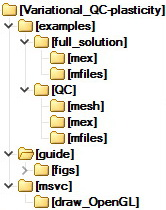
\includegraphics[scale=0.75]{figs/folders.jpg}
	\caption{File system of downloaded repository.}
	\label{Sect:2:Fig:1}
\end{figure}
%

Concerning the implementation itself, sub-folders \texttt{full\_solution} and \texttt{QC}, both inside the \texttt{examples} folder, directly contain MATLAB m-files that serve to run one of the two examples. These are named as \texttt{RUN\_*.m}. Other m-files, collected in \texttt{mfiles} sub-folders, are supporting and serve, e.g., to construct a mesh or to minimize the potential energy with respect to~$\bs{r}$. MATLAB mex functions, gathered inside \texttt{mex} sub-folders, are provided to improve the overall performance. In order to run any example, all included mex-files \emph{must be} compiled first, cf. Section~\ref{SubSect:3.1}.

The \texttt{msvc} sub-folder comprises an optional post-processing tool that helps to view computed results (available only for pc). Its source code and Microsoft Visual Studio (MSVC) 2013 project files are contained in \texttt{draw\_OpenGL} folder; compilation procedure is detailed in Section~\ref{SubSect:3.2} 
%
%-----------------------------------------------------------------------------
%	SECTION 3
%-----------------------------------------------------------------------------
%
\section{Compilation}
\label{Sect:3}
%
%---------------------------------
%	SUBSECTION 3.1
%---------------------------------
%
\subsection{REQUIRED: Basic Compilation}
\label{SubSect:3.1}
%
In order to compile, a C++ compiler has to be present on the local machine. For the list of supported and compatible compilers refer \href{https://www.mathworks.com/support/compilers/}{here}.

As a next step, installed compiler must be linked to MATLAB. This is done by executing \texttt{mex -setup C++} in MATLAB's command window, which prints available compilers: choosing one of them completes the linking process. Note that if a compiler is already linked, the message indicating its type and version will be printed. If an error occurs, the compiler has not been installed properly. In that case please follow the recommended procedures for the proper installation of particular compiler in your operating system (OS).

If a compiler is successfully installed, or was already present on the local machine, run \texttt{examples/\allowbreak full\_solution/\allowbreak compile\_mex.m} and \texttt{examples/\allowbreak QC/\allowbreak compile\_mex\_QC.m} in order to compile provided source files.

The implementation has been tested using Matlab~2016a and Microsoft Visual studio~2013 on pc (Windows), gcc~5.4.0 on unix, and Xcode~7.3.1 on mac.
%
%---------------------------------
%	SUBSECTION 3.2
%---------------------------------
%
\subsection{OPTIONAL: Drawing Tool (for pc only)}
\label{SubSect:3.2}
%
Applies for MSVC only: first download \href{http://freeglut.sourceforge.net/}{freeglut}, \href{http://glew.sourceforge.net/}{glew}, and \href{http://glui.sourceforge.net/}{glui} packages, unpack them and build solutions whenever necessary (this routine was verified for freeglut~3.0.0.1, glew 1.13.0, glui~2.35, and MSVC~2013).

In order to compile glui, open \texttt{glui/src/msvc/glui.sln} in MSVC. First change \emph{Solution Configurations} to \emph{Release} and set to x64 if necessary (\emph{Configuration manager} $\rightarrow$ \emph{Platform} $\rightarrow$ \emph{New} $\rightarrow$ \emph{x64}). In \emph{Solution Explorer}, right-click on \emph{\_glui library} and go to \emph{Properties} $\rightarrow$ \emph{VC++ Directories}, where in \emph{Include Directories} add \texttt{freeglut/include} directory. Subsequently, right-click on \emph{\_glui library} and \emph{Build}. 

Open \texttt{codes\_plasticity/msvc/draw\_OpenGL/draw\_OpenGL.sln}. Perhaps, a conversion to a newer MSVC version will be required since \texttt{*.sln} file was created for MSVC~2013. In \emph{Configuration manager} select \emph{Win32} or \emph{x64} for \emph{Solution Platforms}, and choose \emph{Release} in \emph{Solution Configurations}. Go to \emph{Solution Explorer}, right-click on \emph{draw\_OpenGL}, go to \emph{Properties} $\rightarrow$ \emph{VC++ Directories}, where in \emph{Include Directories} add \texttt{freeglut/include}, \texttt{glew/include}, and \texttt{glui/src/include}. Press apply. In \emph{Library Directories} add \texttt{freeglut/ lib} (or \texttt{freeglut/lib/x64}), \texttt{glew/lib/Release/x*}, and \texttt{glui/src/msvc/lib}; choose always those libraries that match your OS, i.e. x86 or x64. Press apply and go to \emph{Linker} $\rightarrow$ \emph{Input} $\rightarrow$ \emph{Additional Dependencies} and here enter \texttt{freeglut.lib} (press enter for a new line), \texttt{glew32.lib}, and \texttt{glui32.lib}. Press \emph{OK}, \emph{Apply}, and \emph{OK}. Now, the solution can be built: \emph{Build} $\rightarrow$ \emph{Build Solution}.

Having successfully built the solution, go to \texttt{codes\_plasticity/msvc/draw\_OpenGL/ Release} (or to \texttt{codes\_plasticity/msvc/draw\_OpenGL/x64/Release}) and copy \texttt{draw\_OpenGL.exe} to the folder where \texttt{RUN\_*.m} files are situated. Further, it is necessary to copy also \texttt{freeglut.dll} file from \texttt{freeglut/bin} and \texttt{glew32.dll} from \texttt{glew/bin/Release} to this location, since \texttt{draw\_OpenGL.exe} uses them. Again, match your OS type.

Before execution of \texttt{call\_OpenGL.mex} and \texttt{draw\_OpenGL.exe}, scripts \texttt{RUN\_*.m} automatically test for all the required files. Therefore, until all libraries and executables are present, the results will not be displayed.

The entire post-processor implementation is contained in one source file, \texttt{draw\_OpenGL.cpp}, described briefly in Section~\ref{Sect:5}.
%
%-----------------------------------------------------------------------------
%	SECTION 5
%-----------------------------------------------------------------------------
%
\section{Description of the Implementation}
\label{Sect:5}
%
Each file or external function used during the solution process is shortly described below in this section. Namely, variables which can be adjusted such as problem dimensions, solver tolerances, mesh generators, or various flags are specified; further details can be found as comments in source files.

For convenience, we recall the full-lattice version of the AM algorithm in Algorithm~\ref{Sect:5:Alg:1}. Here, two auxiliary variables~$\widetilde{\bs{r}}$ and~$\widetilde{\bs{z}}_\mathrm{p}$ are introduced. Note that superscript symbols~$(i)$ and~$[l]$ relate to Newton iterations in the case of~$(i)$ or~$(j)$, and to AM iterations in the case of~$[l]$. The symbols~$(\mathrm{end})$ or~$[\mathrm{end}]$ denote appropriate converged quantities at the end of the iteration process. The remaining notation is explained in~\cite[Section~2.2.1]{RokosQC}.\\
%
\begin{singlespace}
	\begin{algorithm}
		\caption{Alternating minimization algorithm.}
		\label{Sect:5:Alg:1}
		\SetKwInOut{Input}{Data}
		\SetKwInOut{Output}{Result}
		\Input{definition of energies, boundary conditions, and tolerances; initial conditions for internal variables are set to~$\bs{0}$}
		\Output{evolution of state variables~$\bs{r}$, $\bs{z}_\mathrm{p}$, and~$\bs{z}_\mathrm{c}$ as functions of time~$t_k$, $k=1,\dots,n_T$}
		initialize~$\bs{r}(t_0):=\bs{r}_0$, $\bs{z}_\mathrm{p}(t_0):=\bs{0}$, $\bs{z}_\mathrm{c}(t_0):=\bs{0}$\\
		\For{$k:=1$ \KwTo $n_T$}{
			initialize~$\widetilde{\bs{r}}^{[0](\mathrm{end})}:=\bs{r}(t_{k-1})$, $\widetilde{\bs{z}}_\mathrm{p}^{[0](\mathrm{end})}:=\bs{z}_\mathrm{p}(t_{k-1})$,  $\varepsilon_{\mathrm{alt}}:=\mathrm{tol_{alt}}+1$\\
			\nonl {\color{ForestGreen}\% perform the AM procedure:}\\
			set~$l:=0$\\
			\While{$\varepsilon_{\mathrm{alt}}>\mathrm{tol_{alt}}$}{
				initialize~$\widetilde{\bs{r}}^{[l+1](0)}:=\widetilde{\bs{r}}^{[l](\mathrm{end})}$, $\widetilde{\bs{z}}_\mathrm{p}^{[l+1](0)}:=\widetilde{\bs{z}}_\mathrm{p}^{[l](\mathrm{end})}$\\
				\nonl {\color{ForestGreen}\% minimize~$\Pi_\mathrm{red}^k(\widehat{\bs{r}},\widetilde{\bs{z}}_\mathrm{p}^{[l+1](0)};\bs{z}_\mathrm{p}(t_{k-1}),\bs{z}_\mathrm{c}(t_{k-1}))$ with respect to~$\widehat{\bs{r}}$:}\\
				set~$i:=0$, initialize~$\bs{f}_{\bs{r}}^{(0)}:=-\partial\Pi(\bs{r})/\partial\bs{r}|_{\bs{r}=\widetilde{\bs{r}}^{[l+1](0)}}$\\ 
				\While{$||\bs{f}^{(i)}_{\bs{r}}||_2>\mathrm{tol}_\bs{r}$}{
					$\bs{K}_{\bs{r}}^{(i)}:=\partial^2\Pi(\bs{r})/\partial\bs{r}\partial\bs{r}|_{\bs{r}=\widetilde{\bs{r}}^{[l+1](i)}}$\\ 
					$\widetilde{\bs{r}}^{[l+1](i+1)}:=\widetilde{\bs{r}}^{[l+1](i)}+(\bs{K}_{\bs{r}}^{(i)})^{-1}\bs{f}_{\bs{r}}^{(i)}$\\
					update~$\bs{f}_{\bs{r}}^{(i+1)}:=-\partial\Pi(\bs{r})/\partial\bs{r}|_{\bs{r}=\widetilde{\bs{r}}^{[l+1](i+1)}}$\\
					set~$i:=i+1$\\}
				\nonl {\color{ForestGreen}\% minimize~$\Pi_\mathrm{red}^k(\widetilde{\bs{r}}^{[l+1](\mathrm{end})},\widehat{\bs{z}}_\mathrm{p};\bs{z}_\mathrm{p}(t_{k-1}),\bs{z}_\mathrm{c}(t_{k-1}))$ with respect to~$\widehat{\bs{z}}_\mathrm{p}$:}\\
				set~$j:=0$, initialize~ $\bs{f}_{\bs{z}}^{(0)}:=-\partial\Pi(\bs{z}_\mathrm{p})/\partial\bs{z}_\mathrm{p}|_{\bs{z}_\mathrm{p}=\widetilde{\bs{z}}_\mathrm{p}^{[l+1](0)}}$\\ 
				\While{$||\bs{f}^{(j)}_{\bs{z}}||_2>\mathrm{tol}_\bs{z}$}{
					\nonl
					{\color{ForestGreen}\% Newton's method either for smoothing or return-mapping algorithm with non-linear hardening}\\
					$\bs{K}_{\bs{z}}^{(j)}:=\partial^2\Pi(\bs{z}_\mathrm{p})/\partial\bs{z}_\mathrm{p}\partial\bs{z}_\mathrm{p}|_{\bs{z}_\mathrm{p}=\widetilde{\bs{z}}_\mathrm{p}^{[l+1](j)}}$\\ 
					$\widetilde{\bs{z}}_\mathrm{p}^{[l+1](j+1)}:=\widetilde{\bs{z}}_\mathrm{p}^{[l+1](j)}+(\bs{K}_{\bs{z}}^{(j)})^{-1}\bs{f}_{\bs{z}}^{(j)}$\\
					update~$\bs{f}_{\bs{z}}^{(j+1)}:=-\partial\Pi(\bs{z}_\mathrm{p})/\partial\bs{z}_\mathrm{p}|_{\bs{z}_\mathrm{p}=\widetilde{\bs{z}}_\mathrm{p}^{[l+1](j+1)}}$\\
					set~$j:=j+1$\\}
				$\varepsilon_{\mathrm{alt}}:=||\widetilde{\bs{z}}_\mathrm{p}^{[l+1](\mathrm{end})}-\widetilde{\bs{z}}_\mathrm{p}^{[l](\mathrm{end})}||_2$\\
				set~$l:=l+1$\\
			}
			$\bs{r}(t_{k}):=\widetilde{\bs{r}}^{[\mathrm{end}](\mathrm{end})}$, $\bs{z}_\mathrm{p}(t_{k}):=\widetilde{\bs{z}}_\mathrm{p}^{[\mathrm{end}](\mathrm{end})}$,\\
			$\bs{z}_\mathrm{c}(t_{k}):=\bs{z}_\mathrm{c}(t_{k-1})+|\bs{z}_\mathrm{p}(t_{k})-\bs{z}_\mathrm{p}(t_{k-1})|$\\
		}
	\end{algorithm}
\end{singlespace}
%
%---------------------------------
%	SUBSECTION 5.1
%---------------------------------
%
\subsection{Description of \texttt{\emph{*.m}} files}
\label{SubSect:5.1}
%
%-------- SUBPARAGRAPH --------%
%
\subparagraph{RUN\_uniform\_loading} executes the full-lattice simulation for the uniform loading case, see~\cite[Section~5.1]{RokosQC}. First, MATLAB is reset to its initial configuration, memory is wiped, and working paths are initialized. Subsequently, the script loads user-defined parameters specifying geometry, material data, constructs \texttt{atoms} and \texttt{bonds} databases (cf. Section~\ref{SubSect:5.2}), and assembles boundary conditions. The AM algorithm subsequently minimizes the energy through iterative execution of \emph{minimize\_r} and \emph{return\_mapping} functions for each time step~$t_k$, until convergence is reached. Finally, results are shown: deformed configuration, energy evolution paths, or the post-processing step through \emph{call\_OpenGL} function is executed, if available.

The following list of input constants allows to adjust the example: \texttt{dSizeX} and~\texttt{dSizeY} describe lattice spacings along~$x$- and~$y$-axes, \texttt{SizeX} and~\texttt{SizeY} describe one half of the rectangular domain~$\Omega_0$ along~$x$- and~$y$-axes, \texttt{RigidX} and~\texttt{RigidY} describe one halves of the central inclusion along~$x$- and~$y$-axes. $\texttt{PotentialI}=[E_\mathrm{I},H_\mathrm{I},\sigma_{0,\mathrm{I}},\rho_\mathrm{I}]$, $\texttt{PotentialM}=[E_\mathrm{M},H_\mathrm{M},\sigma_{0,\mathrm{M}},\rho_\mathrm{M}]$ characterise material parameters of the inclusion and surrounding matrix. \texttt{TOL\_am}, \texttt{TOL\_r}, \texttt{TOL\_z}, and \texttt{TOL\_g} specify relative error tolerances for the AM algorithm, for the Newton's method with respect to~$\bs{r}$, for the Newton's method used during the return-mapping algorithm when~$\bs{z}_\mathrm{p}$ variable is being computed, and the geometric tolerance (a distance that is smaller than \texttt{TOL\_g} is treated as zero). Dirichlet boundary conditions, namely $x$-displacement magnitude of~$\Gamma_2$, is specified in~\texttt{u\_D}. Pseudo-time profile and the number of time increments~$n_T$ can be adjusted in~\texttt{Time} variable. Concerning basic outputs, the \texttt{scale} variable prescribes the magnification factor of the displacements for the final deformed configuration. Above, Young's modulus~$E$, hardening modulus~$H$, initial yield stress~$\sigma_0$, and hardening exponent~$\rho$ specify particular physical parameters of the lattice.
%
%-------- SUBPARAGRAPH --------%
%
\subparagraph{RUN\_pure\_bending} provides the solution of the pure bending example presented in~\cite[Section~5.2]{RokosQC} for the full-lattice formulation. Structure of the code is identical to the one in \texttt{RUN\_uniform\_loading.m} file; several marginal differences in formulation of boundary conditions occur, however. In particular, \texttt{RigidY} describes the entire size of the bottom-edge inclusion along $y$-axis instead of one half; instead of~\texttt{u\_D}, the parameter~\texttt{THETA} specifies target deformation.
%
%-------- SUBPARAGRAPH --------%
%
\subparagraph{RUN\_indentation} solves the example presented in~\cite[Section~5.3]{RokosQC} for the full-lattice formulation. Structure of the code is identical to the two previous ones, \texttt{RUN\_uniform\_loading.m} and \texttt{RUN\_pure\_bending.m}. The only differences are in the formulation of the boundary conditions, used minimization procedure, and in presence of two new parameters specifying the indenter. Regarding boundary condition, all three parts of the boundary~$\Gamma_{1,2,4}$ are fixed in horizontal as well as vertical direction, whereas~$\Gamma_3$ is left free. Here, contact with the indenter is assumed. The position of the indenter is specified through its centre~\texttt{C} which depends on \texttt{Time}. In order to minimize~$\Pi^k_\mathrm{red}$ with respect to kinematic variables, function \emph{minimize\_r\_I} or \emph{minimize\_r\_ISQP} is called, which incorporates inequality constraints through Lagrange multipliers and active-set strategy. The new parameters are string \texttt{indenter}, which specifies indenter's profile ("square" or "circular"), and \texttt{Rind}, which specifies its size (half-side of the square or radius of the circular indenter). Because the specimen is homogeneous, only one~$\texttt{Potential}=[E,H,\sigma_{0},\rho]$ characterizes material properties.
%
%-------- SUBPARAGRAPH --------%
%
\subparagraph{grad\_hess} provides the full vector~$\bs{r}$ denoted as~\texttt{r2} (which is reconstructed from the current iteration variable~$\bs{x}$), and gradient and Hessian of the reduced incremental energy~$\Pi^k_\mathrm{red}$ for the full-lattice system with respect to~$\bs{r}$. This function effectively reduces to the execution of the \emph{build\_grad\_r} and \emph{build\_hess\_r} procedures followed by the application of prescribed Dirichlet boundary conditions.
%
%-------- SUBPARAGRAPH --------%
%
\subparagraph{minimize\_r} executes the minimization step~(AMa) with respect to~$\bs{r}$ at a fixed time step~$t_k$ and AM iteration~$l$. First, \emph{grad\_hess} function is called to provide the gradient, Hessian, and current-iteration configuration~$\bs{r}$. Then, tying conditions are introduced and the saddle point problem assembled and solved. Convergence of the Newton's algorithm is achieved when relative error is smaller than~\texttt{TOL\_r}. After convergence, full vector~$\bs{r}^{[l]}(t_k)$, denoted as~\texttt{r2}, is returned together with the number of Newton iterations~\texttt{Niter}.
%
%-------- SUBPARAGRAPH --------%
%
\subparagraph{minimize\_r\_I} minimizes the incremental energy with respect to kinematic variable~$\bs{r}$ in the~AM algorithm, cf. \emph{minimize\_r}. Contrary to \emph{minimize\_r}, inequality constraints are incorporated through primal-dual formulation and active-set strategy. 

Atoms that may come into contact with the indenter (and are therefore tested for penetration) are stored in \texttt{IDGamma\_3} array. Indices of those from \texttt{IDGamma\_3} that actually are in the contact are listed in \texttt{IDActive}. For each atom in \texttt{IDActive}, associated inequality constraint is enforced as equality constraint (linear for square and nonlinear for circular indenter). Subsequently, Newton's algorithm is iterated until convergence. Upon convergence, active set is updated and if necessary, the system is relaxed again until both, \texttt{IDActive} set and Newton's algorithm converge. Function \emph{minimize\_r\_I} returns amongst others \texttt{IDActive} array that is used as the initial estimate for the next step or AM iteration.
%
%-------- SUBPARAGRAPH --------%
%
\subparagraph{minimize\_r\_ISQP} works as an alternative to \emph{minimize\_r\_I}. In order to deal with inequality constraints, this function employs the Sequential Qudaratic Programming~(SQP) algorithm along with active set strategy. Further details on SQP and active set can be found e.g. in~\cite{Fletcher:1987:PMO,BonnansOptim,Nocedal:2006:NumOpt}.
%
%-------- SUBPARAGRAPH --------%
%
\subparagraph{RUN\_uniform\_loading\_QC} solves the uniform loading example using the QC approach. Apart from the procedures contained in \texttt{RUN\_uniform\_loading.m}, two additional steps have to be accomplished. Firstly, for the interpolation, the domain~$\Omega_0$ has to be triangulated. Here, four options are offered: (1)~load one of the meshes presented in~\cite[Fig.~5]{RokosQC} and provided in the \texttt{mesh} folder; (2)~build a regular mesh using right-triangulated irregular networks (RTIN) and longest-edge-propagation-path (LEPP) refinement algorithm after~\cite{Rivara:LEPP}; (3)~build a mesh using~\href{http://ksm.fsv.cvut.cz/~dr/t3d.html}{$\mathcal{T}3\mathcal{D}$} generator through \emph{mesh\_T3d\_QC}; (4)~call the MATLAB mesh generator \emph{initmesh} through \emph{mesh\_MATLAB\_QC}. Secondly, for the summation rule, the database of sampling atoms is specified through \emph{sort\_sampling\_atoms\_QC} function. Boundary and tying conditions for repatoms are finally provided by \texttt{build\_phi\_u\_QC.m}.

In comparison with the full solution \emph{RUN\_uniform\_loading}, couple of additional variables have to be specified. \texttt{SumRule} characterises summation rule to be used: 0~for the exact summation rule, 1~for the central summation rule (both after Beex~\emph{et al.}), and 2~for the full summation rule. \texttt{MeshType} specifies domain triangulation to be used: 0~for using one of the provided meshes, 1~for using RTIN mesh, 2~for using the \href{http://ksm.fsv.cvut.cz/~dr/t3d.html}{$\mathcal{T}3\mathcal{D}$} generator, and 3~for using the MATLAB mesh generator. Finally, \texttt{FineX} and \texttt{FineY} describe half sizes of the fully-resolved mesh region along~$x$- and~$y$-axes.
%
%-------- SUBPARAGRAPH --------%
%
\subparagraph{RUN\_pure\_bending\_QC} solves the pure bending example using the QC approach; for completeness, refer also to \emph{RUN\_uniform\_loading\_QC} and \emph{RUN\_uniform\_loading}. Four options for the interpolation step are provided again: use stored meshes described in~\cite[Fig.~9]{RokosQC}, RTIN, \href{http://ksm.fsv.cvut.cz/~dr/t3d.html}{$\mathcal{T}3\mathcal{D}$}, or MATLAB. 

Contrary to \emph{RUN\_uniform\_loading\_QC} function, \texttt{RigidY} now describes the entire size of the bottom-edge inclusion along the $y$-axis instead of one half; analogously for~\texttt{FineY}. Instead of~\texttt{u\_D}, which specifies the Dirichlet boundary conditions, angle~\texttt{THETA} is prescribed. 
%
%-------- SUBPARAGRAPH --------%
%
\subparagraph{RUN\_indentation\_QC} provides results for the indentation example using QC approach. Functions \emph{minimize\_r\_I\_QC} or \emph{minimize\_r\_ISQP\_QC} minimize the incremental energy with respect to kinematic variable, cf. \emph{RUN\_indentation}.
%
%-------- SUBPARAGRAPH --------%
%
\subparagraph{grad\_hess\_QC} provides current-iteration vector~$\bs{r}_\mathrm{rep}$, denoted as~\texttt{r2}, together with the gradient and Hessian of the approximate incremental energy~$\widehat{\Pi}^k_\mathrm{red}$ with respect to the reduced variable~$\bs{r}_\mathrm{rep}$. In the function call, first the full vector~$\bs{r}$ is reconstructed through the interpolation matrix~$\bs{\Phi}$. Then, using chosen summation rule, full-dimensional approximate gradient and Hessian are computed through \emph{build\_grad\_r\_QC} and \emph{build\_hess\_r\_QC} mex-functions. Finally, the reduction step is carried out through the interpolation matrix~$\bs{\Phi}$ and the Dirichlet boundary conditions are prescribed.
%
%-------- SUBPARAGRAPH --------%
%
\subparagraph{minimize\_r\_QC} minimizes the approximate reduced incremental energy~$\widehat{\Pi}^k_\mathrm{red}$ with respect to~$\bs{r}_\mathrm{rep}$. Iteratively, \emph{grad\_hess\_QC} function is called to provide the reduced gradient and Hessian, followed by incorporation of the tying conditions for~$\bs{r}_\mathrm{rep}$ to yield the saddle point problem, cf. also \emph{minimize\_r}. Converged vectors~$\bs{r}_\mathrm{rep}$ and~$\bs{r}$, denoted as~\texttt{r2} and~\texttt{r}, and the number of Newton iterations~\texttt{Niter} are returned. 
%
%-------- SUBPARAGRAPH --------%
%
\subparagraph{minimize\_r\_I\_QC} minimizes the approximate incremental energy with respect to kinematic variable, see also \emph{minimize\_r\_QC}. This function is extended to reflect also inequality constraints due to indenter. Used strategy is the same as in \emph{minimize\_r\_I}, applied only to repatoms instead of to all atoms.
%
%-------- SUBPARAGRAPH --------%
%
\subparagraph{minimize\_r\_ISQP\_QC} is an alternative to~\emph{minimize\_r\_QC}. In analogy to \emph{minimize\_r\_ISQP}, this function employs SQP algorithm with active set strategy.
%
%-------- SUBPARAGRAPH --------%
%
\subparagraph{mesh\_MATLAB\_QC} depending on the example type (uniform loading or pure bending), this function assembles required inputs to MATLAB \emph{initmesh} function, and subsequently generates the mesh. Since all the mesh nodes have to spatially conform to the underlying lattice, node coordinates are rounded with respect to \texttt{dSizeX} and \texttt{dSizeY} and the resulting mesh is checked for hanging nodes in \texttt{RUN\_*.m}. Function returns an array of final triangles~\texttt{t} and an array of node points~\texttt{p}. For the definition of \texttt{t} and \texttt{p} see MATLAB help for the keyword \emph{initmesh}. Note that as an alternative to this approach, one could use Delaunay triangulation. In that case, repatoms have to be chosen carefully.

\texttt{HMax} variable limits longest edges of triangles.  
%
%-------- SUBPARAGRAPH --------%
%
\subparagraph{mesh\_T3d\_QC} depending on the example type, this function assembles an input file \texttt{T3d.in} for the \href{http://ksm.fsv.cvut.cz/~dr/t3d.html}{$\mathcal{T}3\mathcal{D}$} mesh generator. Subsequently, \texttt{T3d.exe} routine with several options is called; for a closer description of this program and its download please refer \href{http://mech.fsv.cvut.cz/~dr/software/T3d/guide.pdf}{here}. \href{http://ksm.fsv.cvut.cz/~dr/t3d.html}{$\mathcal{T}3\mathcal{D}$} generates an output file called \texttt{T3d.out}, which is parsed and converted to~\texttt{p} and~\texttt{t} arrays. Then, node coordinates are rounded with respect to \texttt{dSizeX} and \texttt{dSizeY}.
%
%-------- SUBPARAGRAPH --------%
%
\subparagraph{mesh\_RTIN\_QC} takes as inputs constants specifying the sizes of the rectangular domain and finely refined region, and returns the triangulations represented by point and triangle matrices \texttt{p} and \texttt{t}. Initially, a coarse regular mesh is constructed, which is iteratively (by calling \emph{regular\_refine}) refined until all required points of the fully-resolved region become repatoms.
%
%-------- SUBPARAGRAPH --------%
%
\subparagraph{regular\_refine} refines current triangulation according to specified set of triangles marked for refinement, \texttt{refine\_triangles}. The fully refined triangles are first excluded from the list, \emph{refine\_mesh} algorithm subsequently performs actual mesh refinement. Matrices \texttt{p} and \texttt{t}, that represent refined triangulation, are returned.
%
%---------------------------------
%	SUBSECTION 5.2
%---------------------------------
%
\subsection{Description of \texttt{\emph{*.cpp}} mex-files}
\label{SubSect:5.2}
%
%-------- SUBPARAGRAPH --------%
%
\subparagraph{build\_atoms} serves first to build the database of atoms, i.e. to provide a system of structures

\noindent
\texttt{\begin{tabular}{@{}r@{}l@{}}
atoms($\alpha$) & .R(2) \\
& .NeighbourList(n) \\
& .BondList(n)
\end{tabular}}

\noindent
for~$\alpha=1,\dots,n_\mathrm{ato}$, where~$\texttt{R}=[r_{0,x},r_{0,y}]$, and \texttt{NeighbourList} is an \texttt{n}-dimensional vector, storing IDs of atoms contained in the set~$B_\alpha$; note that~$\texttt{n} = \# B_\alpha$. Similarly, \texttt{BondList}, also an array of the length~$\# B_\alpha$, is allocated to store IDs of bonds connecting an atom~$\alpha$ with its nearest neighbours stored in~$B_\alpha$, yet left empty. Bond IDs are supplied later by \emph{build\_bonds} function call. Note that the array~$\texttt{R0}=[\bs{r}_0^1,\dots,\bs{r}_0^{n_\mathrm{ato}}]^\mathsf{T}$, $\texttt{R0}(2\alpha-1,2\alpha)=[r_{0,x}^\alpha,r_{0,y}^\alpha]^\mathsf{T}$, i.e. the vector of all atoms' initial positions, can be constructed as $\texttt{R0} = [\texttt{atoms(:).R}]'$.

As an input, the array $[\texttt{SizeX},\allowbreak\texttt{SizeY},\allowbreak\texttt{dSizeX},\allowbreak\texttt{dSizeY}]$ storing dimensions of the problem has to be supplied. It represents a rectangular domain~$\Omega_0 = [-\texttt{SizeX},\allowbreak\texttt{SizeX}]\times [-\texttt{SizeY},\allowbreak\texttt{SizeY}]$ with atom spacings~\texttt{dSizeX} along~$x$- and~\texttt{dSizeY} along $y$-axes.
%
%-------- SUBPARAGRAPH --------%
%
\subparagraph{build\_bonds} provides the database of bonds, i.e.

\noindent
\texttt{\begin{tabular}{@{}r@{}l@{}}
bonds($m$) & .Atoms(2) \\
& .Potential(4) \\
\end{tabular}}

\noindent
for~$m = 1,\dots,n_\mathrm{bon}$. Each bond connects atoms~$\alpha$ and~$\beta$ stored in $\texttt{Atoms}=[\alpha,\beta]$, and has material parameters specified in~$\texttt{Potential}=[E^{\alpha\beta},H^{\alpha\beta},\sigma_0^{\alpha\beta},\rho^{\alpha\beta}]$. Possible reduction of cross-sectional bond area is accomplished by scaling~$E$ and~$\sigma_0$. This function provides also~$\texttt{atoms}(\alpha).\texttt{BondList}$ for each~$\alpha$, discussed in \emph{build\_atoms} function description. Although in the context of homogeneous lattice structures this kind of representation is far from efficient, it is convenient for the representation of inhomogeneous or random structures.
	
As an input, following variables have to be provided: \texttt{atoms}, $[\texttt{SizeX},\allowbreak\texttt{SizeY},\allowbreak\texttt{dSizeX},\allowbreak\texttt{dSizeY},\allowbreak\texttt{RigidX},\allowbreak\texttt{RigidY}]$, \texttt{PotentialI}, \texttt{PotentialM}, \texttt{flag}, and \texttt{TOL\_g}. For the definition of \texttt{atoms} and $[\texttt{SizeX},\allowbreak\texttt{SizeY},\allowbreak\texttt{dSizeX},\allowbreak\texttt{dSizeY}]$ refer to \emph{build\_atoms}. \texttt{RigidX} and \texttt{RigidY} describe the rigid inclusion's dimensions having the material parameters stored in \texttt{PotentialI}. \texttt{PotentialM} specifies the material parameters assigned to the surrounding matrix; both inputs are structured as $\texttt{PotentialI}=[E_\mathrm{I},H_\mathrm{I},\sigma_{0,\mathrm{I}},\rho_\mathrm{I}]$, $\texttt{PotentialM}=[E_\mathrm{M},H_\mathrm{M},\sigma_{0,\mathrm{M}},\rho_\mathrm{M}]$. Variable \texttt{flag} chooses the location of the inclusion: 0~for the central inclusion, 1~for the bottom-edge inclusion. The last input parameter is \texttt{TOL\_g}, set as default to~$10^{-10}$. When algorithm decides which atoms belong to the inclusion~$\mathscr{I}$, it first computes the $\ell_1$-distance $\mathrm{dist}(\bs{r}_0^\alpha,\mathscr{I})$ between the position vector~$\bs{r}_0^\alpha$ and the inclusion~$\mathscr{I}$. Therefore, if $\mathrm{dist}(\bs{r}_0^\alpha,\mathscr{I})<\texttt{TOL\_g}$, then~$\alpha\in\mathscr{I}$. Bond~$\alpha\beta\in\mathscr{I}$ if~$\alpha\in\mathscr{I}$ and~$\beta\in\mathscr{I}$ at the same time.
%
%-------- SUBPARAGRAPH --------%
%
\subparagraph{build\_grad\_r} returns a vector~\texttt{f\_r} storing the first derivatives of the incremental energy with respect to~$\bs{r}$, i.e.~$\texttt{f\_r}=\partial\Pi^k_\mathrm{red}/\partial\bs{r}=\partial\mathcal{V}^\mathrm{int}/\partial\bs{r}$. As inputs, \texttt{atoms}, \texttt{bonds}, \texttt{r}, and \texttt{z} variables have to be provided. Here, \texttt{atoms} is the database of all atoms, \texttt{bonds} the database of all bonds, $\texttt{r}=[\bs{r}^1,\dots,\bs{r}^{n_\mathrm{ato}}]^\mathsf{T}$, $\texttt{r}(2\alpha-1,2\alpha)=[r_x^\alpha,r_y^\alpha]^\mathsf{T}$ stores current positions of all atoms~$\alpha=1,\dots,n_\mathrm{ato}$ (and represents the counterpart to~$\widetilde{\bs{r}}$ variable in Algorithm~\ref{Sect:5:Alg:1}), whereas $\texttt{z}=[z_p^1,\dots,z_p^{n_\mathrm{bon}}]^\mathsf{T}$ stores plastic slips for all bonds~$\alpha\beta$, being the counterpart to~$\widetilde{\bs{z}}_\mathrm{p}$.
%
%-------- SUBPARAGRAPH --------%
%
\subparagraph{build\_hess\_r} returns three two-dimensional full matrices~\texttt{I}, \texttt{J}, and~\texttt{S} storing row indices, column indices, and values of the Hessian. In other words, this function provides the so-called COO sparse matrix representation of the Hessian. Employing MATLAB's function~$\texttt{K\_r} = \allowbreak \emph{sparse}(\texttt{I(:)},\texttt{J(:)},\texttt{K(:)},\texttt{n},\texttt{n})$ for vectorised matrices~\texttt{I}, \texttt{J}, and~\texttt{K}, a sparse $\texttt{n}\times\texttt{n}$ matrix representing the global Hessian of the reduced incremental energy, $\Pi^k_\mathrm{red}$, with respect to~$\bs{r}$ is computed, i.e.~$\texttt{K\_r}=\partial^2\Pi^k_\mathrm{red}/\partial\bs{r}\partial\bs{r}=\partial^2\mathcal{V}^\mathrm{int}/\partial\bs{r}\partial\bs{r}$; above, $\texttt{n} = 2n_\mathrm{ato}$. For further details on assembling stiffness matrices in MATLAB see~\cite{Stiffness}. As an input, \texttt{atoms} and \texttt{bonds} databases have to be provided as well as the vector of current atoms' positions~\texttt{r} and plastic deformations~\texttt{z}. See \emph{build\_grad\_r} paragraph for the definitions of~\texttt{r} and~\texttt{z}.
%
%-------- SUBPARAGRAPH --------%
%
\subparagraph{return\_mapping} performs the minimization step~(AMb), i.e. minimizes the reduced incremental energy~$\Pi^k_\mathrm{red}$ with respect to internal variables~$\bs{z}_\mathrm{p}$ at a fixed time step and AM iteration, $t_k$ and~$l$. This function returns a vector of plastic deformations, denoted as~\texttt{z2}. Rewriting~$\Pi^k_\mathrm{red}$ in the bond-wise form, this amounts to independent minimization of each non-smooth bond-energy~$\widetilde{\pi}_m^k(z_\mathrm{p}^m)$ with respect to~$z_\mathrm{p}^m$ for~$m=1,\dots,n_\mathrm{bon}$. As inputs, \texttt{atoms} and \texttt{bonds} databases have to be supplied. Further, updated deformation vector~\texttt{r} as well as previous-time-step internal variables~$\texttt{Z(:,k-1)}=[z_\mathrm{p}^1(t_{k-1}),\allowbreak\dots,\allowbreak z_\mathrm{p}^{n_\mathrm{bon}}(t_{k-1})]^\mathsf{T}$ and~$\texttt{K(:,k-1)}=[z_\mathrm{c}^1(t_{k-1}),\allowbreak\dots,\allowbreak z_\mathrm{c}^{n_\mathrm{bon}}(t_{k-1})]^\mathsf{T}$ are required. Finally, iteration tolerance~\texttt{TOL\_z} specifies relative tolerance of the Newton's algorithm for non-linear hardening rule. For detailed description of the return-mapping algorithm refer e.g. to~\cite[Section~1.4.2]{SimoInelast}.

\texttt{MAXITER} constant determines the maximum number of Newton iterations that can be taken when returning back to yield surface for non-linear hardening rule and a single bond. Default value is set to~100.
%
%-------- SUBPARAGRAPH --------%
%
\subparagraph{build\_en} returns the elastic part~$\mathcal{E}(t_k)$ of the incremental energy~$\Pi^k=\mathcal{E}(t_k)+\mathcal{D}(t_k,t_{k-1})$. As inputs, \texttt{atoms} and \texttt{bonds} databases, atom positions~$\texttt{R(:,k)}=\bs{r}(t_k)$, plastic elongations~$\texttt{Z(:,k)}=\bs{z}_\mathrm{p}(t_k)$, and cumulated plastic elongations~$\texttt{K(:,k)}=\bs{z}_\mathrm{c}(t_k)$ in current time step~$t_k$ have to be provided. For a closer description of~\texttt{Z} and~\texttt{K} refer to \emph{return\_mapping} function.
%
%-------- SUBPARAGRAPH --------%
%
\subparagraph{build\_diss} returns the dissipation part~$\mathcal{D}$ of the incremental energy~$\Pi^k$, i.e. the dissipation distance from the previous to the current time step. Apart from \texttt{atoms} and \texttt{bonds} databases, variables~\texttt{Z(:,k-1)} and~\texttt{Z(:,k)} are required. For their definitions refer to \emph{return\_mapping}.
%
%-------- SUBPARAGRAPH --------%
%
\subparagraph{call\_OpenGL} firstly maps all the resulting data required for the postprocessing step from MATLAB to the OS' memory, i.e. \texttt{atoms}, \texttt{samplingatoms}, \texttt{repatoms}, \texttt{bonds}, \texttt{sampbondsID}, \texttt{triangles}, \texttt{R}, \texttt{Z}, \texttt{K}, \texttt{Time}, \texttt{SizeX}, and \texttt{SizeY}. Subsequently, the secondary process \texttt{draw\_OpenGL.exe} that draws the results is called.
%
%-------- SUBPARAGRAPH --------%
%
\subparagraph{sort\_atoms\_QC} serves to provide five outputs. First, the database of triangles, i.e. an array of structures

\noindent
\texttt{\begin{tabular}{@{}r@{}l@{}}
	triangles(k) & .P1(2) \\
	& .P2(2) \\
	& .P3(2) \\
	& .T(2) \\
	& .IntAtoms(nI) \\			
	& .EdgeAtoms(nE) \\			
	& .VertexAtoms(nV) \\			
	& .NeighTriangles(nN) \\												
\end{tabular}}
	
\noindent
for~$\texttt{k}=1,\dots,\texttt{N{t}}$, where~\texttt{Nt} is the number of triangles, is provided. Above, \texttt{P1}~-- \texttt{P3} store coordinates~$[p_x,p_y]^\mathsf{T}$ of the three vertex atoms or nodes of the \texttt{k}-th triangle, $\texttt{T}=[c_x^\texttt{k},c_y^\texttt{k}]^\mathsf{T}$ stores coordinates of the centroid (or incenter, circumcenter) for the~\texttt{k}-th triangle. \texttt{Int-}, \texttt{Edge-}, and \texttt{Vertex-atoms} store atom IDs of particular atom types; \texttt{VertexAtoms} vector is sorted in correspondence to~\texttt{P1}, \texttt{P2}, and~\texttt{P3}. \texttt{NeighTriangles} collects IDs of all the neighbouring triangles. Second, this function provides a vector~$\texttt{repatoms}= N_\mathrm{rep}^\mathrm{ato}$, that stores all repatoms' IDs. Third, column arrays~\texttt{I}, \texttt{J}, and~\texttt{S} are provided, which store the COO data for~$\bs{\Phi}$ matrix. Using MATLAB's function~$\texttt{Phi}=accumarray([\texttt{I},\texttt{J}],\texttt{S},[2\texttt{n},2\texttt{n\_r}],\mathrm{@max},\mathrm{true})$, a sparse matrix~$\bs{\Phi}$ of size~$2\texttt{n}\times2\texttt{n\_r}$, where~$\texttt{n} = n_\mathrm{ato}$ and~$\texttt{n\_r} = n_\mathrm{rep}$, is computed. As inputs, \texttt{p} and~\texttt{t} matrices (cf. \emph{mesh\_MATLAB\_QC}) along with \texttt{atoms} database and \texttt{TOL\_g} (cf. \emph{RUN\_uniform\_loading}) scalar have to be provided.

Before compilation, user can specify through \texttt{FLAG} which coordinates will be stored in \texttt{T}: 1~for centroid, 2~for incenter, or 3~for circumcenter. Default value is set to~2.
%
%-------- SUBPARAGRAPH --------%
%
\subparagraph{sort\_sampling\_atoms\_QC} provides \texttt{samplingatoms} database, where each entry has the following form

\noindent
\texttt{\begin{tabular}{@{}r@{}l@{}}
	samplingatoms(l) & .ID \\
	& .w \\
	& .List(n) \\
\end{tabular}}

\noindent
for~$\texttt{l}=1,\dots,n_\mathrm{sam}^\mathrm{ato}$, where~\texttt{ID}s are sampling atoms' IDs in \texttt{atoms} database, \texttt{w}s their weight factors, and the variable \texttt{List} stores IDs of atoms that are represented by \texttt{l}-th sampling atom. Required inputs consist of six variables: \texttt{atoms} database, \texttt{triangles} database, \texttt{SumRule} switch specifying the summation rule to be used, $[\texttt{SizeX},\allowbreak \texttt{SizeY}]$ vector describing the domain geometry, \texttt{SW} specifying the example being solved (0~for uniform loading and 1~for pure bending), and \texttt{TOL\_g}. A distance~$\bullet$ for which~$|\bullet|<\texttt{TOL\_g}$ holds is considered as zero; here it serves to locate atoms lying at~$\partial\Omega_0$. Let us recall~\texttt{FLAG} switch from the function \emph{sort\_atoms\_QC}, which specifies whether centroid, 1, incenter, 2, or circumcenter, 3, is stored in~\texttt{T}. In \emph{sort\_sampling\_atoms\_QC}, \texttt{T}~is used as the reference point for choosing the central sampling atom. Atom that is closest to \texttt{T} is chosen. Note, however, that an atom with a higher number of neighbours inside the triangle is chosen preferably. Therefore, the number of neighbours outweighs the distance criterion. 
%
%-------- SUBPARAGRAPH --------%
%
\subparagraph{build\_grad\_r\_QC} serves to compute the gradient of the reduced approximate energy~$\widehat{\Pi}^k_\mathrm{red}$, cf. \emph{build\_grad\_r}; an additional input \texttt{samplingatoms} in contrast to the full gradient has to be provided.
%
%-------- SUBPARAGRAPH --------%
%
\subparagraph{build\_hess\_r\_QC} computes the Hessian of the reduced approximate energy~$\widehat{\Pi}^k_\mathrm{red}$, cf. \emph{build\_hess\_r}; an additional input \texttt{samplingatoms} compared to the full Hessian has to be provided.
%
%-------- SUBPARAGRAPH --------%
%
\subparagraph{return\_mapping\_QC} performs the minimization step~(AMb) of~$\widehat{\Pi}^k_\mathrm{red}$ with respect to~$\bs{z}_{\mathrm{p},\mathrm{sam}}$ at a fixed time step and AM iteration ($t_k$ and~$l$) through the return-mapping algorithm. Function returns~$\bs{z}_{\mathrm{p},\mathrm{sam}}$, stored in fully-dimensional vector~\texttt{z2}; \texttt{samplingbondsID} vector in addition to inputs described in \emph{return\_mapping} is required.
%
%-------- SUBPARAGRAPH --------%
%
\subparagraph{build\_en\_QC} provides the elastic part of the approximate incremental energy~$\widehat{\Pi}^k$ using a summation rule. Besides the inputs specified in \emph{build\_en}, \texttt{samplingatoms} database has to be provided.
%
%-------- SUBPARAGRAPH --------%
%
\subparagraph{build\_diss\_QC} computes dissipation distance part of the approximate incremental energy~$\widehat{\Pi}^k$, cf. also \emph{build\_diss}. This function requires also \texttt{samplingatoms} database in addition to~\texttt{Z(:,k-1)} and~\texttt{Z(:,k)}.
%
%-------- SUBPARAGRAPH --------%
%
\subparagraph{refine\_mesh} performs the Backward-Longest-Edge-Bisection algorithm for a mesh specified by the \texttt{p} and \texttt{t} matrices and for triangles marked for refinement stored in the vector \texttt{refine\_triangles}; for additional details see~\cite{Rivara:LEPP}. Further inputs are switch variable \texttt{SW} and the geometric tolerance \texttt{TOL\_g}. The geometric tolerance serves the usual purpose, i.e. the distance for which~$|\bullet| < \texttt{TOL\_g}$ is treated as zero, whereas the switch decides if the permutation of the \texttt{t} matrix will be verified. If $\texttt{SW}=0$, no permutation takes place. If $\texttt{SW}=1$ indices of each triangle $\texttt{t}(\texttt{:},\texttt{i})$ are checked and permuted such that the first two indices correspond to the longest edge of the triangle. In its fourth row, matrix~\texttt{t} contains IDs of parent elements from the previous mesh; this ID is negative if the triangle was not refined and positive otherwise.

Before compilation, user can specify \texttt{NLEPP} and \texttt{MULT} constants.
\texttt{NLEPP} is the assumed length of the longest-edge-propagation path for the allocation of numerical arrays (default value is 100, though on average achieves value~7). Constant \texttt{MULT} serves to allocate output matrices (\texttt{p} and \texttt{t}). Namely, it tries to predict the ratio of the lengths of inputs to outputs (default value is 10).
%
%---------------------------------
%	SUBSECTION 5.3
%---------------------------------
%
\subsection{Description of \texttt{\emph{*.cpp}} files}
\label{SubSect:5.3}
%
%-------- SUBPARAGRAPH --------%
%
%
\begin{figure}
	\centering
	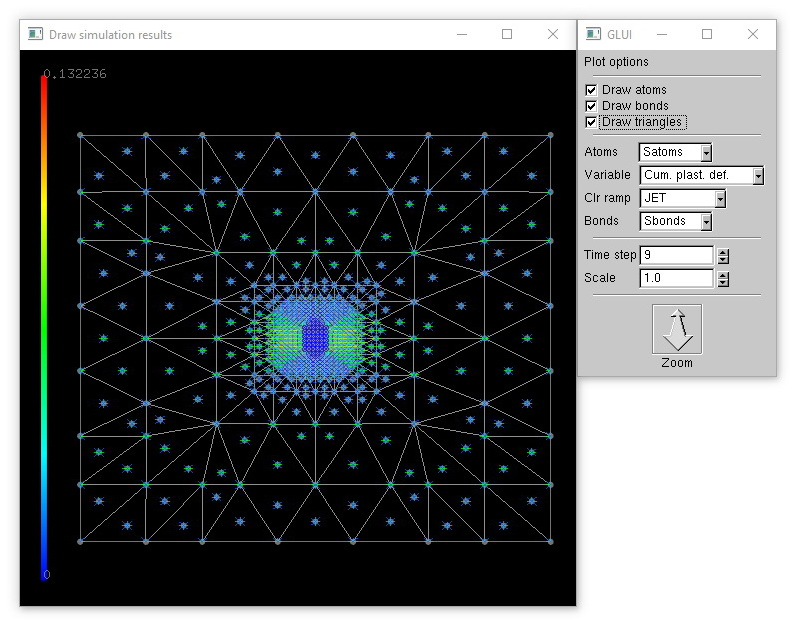
\includegraphics[scale=0.4]{figs/drawing_tool.jpg}
	\caption{A print screen of the drawing tool.}
	\label{SubSect:5.3:Fig:1}
\end{figure}
%
\subparagraph{draw\_OpenGL} closely communicates with \emph{call\_OpenGL} (it is its secondary process). First, data shared by \emph{call\_OpenGL} are assigned and buffered. Subsequently, glut frame with a simple glui menu is initialized and all user's commands are executed. After closing the program, buffers are unmapped such that memory allocated in \emph{call\_OpenGL} can be released. For further details see e.g.~\cite{Hill:OpenGL}. Glui is properly described in it's package manual.

Several options can be set during the program run, cf. Fig.~\ref{SubSect:5.3:Fig:1}. User can draw \emph{atoms}, \emph{bonds}, or \emph{triangles} by marking appropriate checkboxes. Listbox for \emph{Atoms} allows to draw \emph{All atoms}, \emph{Satoms} (sampling atoms), or \emph{Repatoms} (representative atoms). Internal variable that is being plotted is specified in \emph{Variable} listbox, and has two items: \emph{Plastic deformation} for~$\bs{z}_\mathrm{p}$, and \emph{Cum. plast. def.} for~$\bs{z}_\mathrm{c}$. Values of~$\bs{z}_\mathrm{p}$ and~$\bs{z}_\mathrm{c}$ are depicted in four colour schemes specified by listbox \emph{Clr ramp}: \emph{RGB bipolar}, \emph{Thermal}, \emph{JET}, and \emph{RWB}. The set of bonds that will be plotted can be chosen in \emph{Bonds}: \emph{All bonds} or \emph{Sbonds} (sampling bonds). \emph{Time step} spinner serves to choose for which time step~$k$ of~$t_k$ the results will be presented. \emph{Scale} spinner specifies the deformation magnitude ranging from~0 to~100. Finally, drag-icon \emph{Zoom} serves to zoom in or out of the plot. The entire scene can be translated in drag-and-pull manner pressing the left-mouse-button at the same time. Hitting~"$+$" or~"$-$" key will increase or decrease~$k$ of the time step~$t_k$ by one.
%
%% The Appendices part is started with the command \appendix;
%% appendix sections are then done as normal sections
% \appendix
%
%-----------------------------------------------------------------------------
%	APPENDIX A
%-----------------------------------------------------------------------------
%
% \section{XXX}
% \label{Sect:A}
%
%-----------------------------------------------------------------------------
%	APPENDIX B
%-----------------------------------------------------------------------------
%
% \section{YYY}
% \label{Sect:B}
%
%-----------------------------------------------------------------------------
%	ACKNOWLEDGEMENTS
%-----------------------------------------------------------------------------
%
\section*{Acknowledgements}
\addcontentsline{toc}{section}{\numberline{}Acknowledgements}
%
The financial support for this work from the Czech Science Foundation (GA\v{C}R) under project No.~14-00420S is gratefully acknowledged.
%
%-----------------------------------------------------------------------------
%	REFERENCES
%-----------------------------------------------------------------------------
%
\section*{References}
\addcontentsline{toc}{section}{\numberline{}References}
%

%% If you have bibdatabase file and want bibtex to generate the
%% bibitems, please use
%%
\bibliographystyle{abbrvnat}
\bibliography{bibfile}

\end{document}

\endinput
%%
%% End of file `elsarticle-template-harv.tex'.
